\documentclass{standalone}
\usepackage{tkz-base}
\usepackage{tkz-fct}
\usepackage{tkz-euclide}
\usepackage{tikz}
\begin{document}
    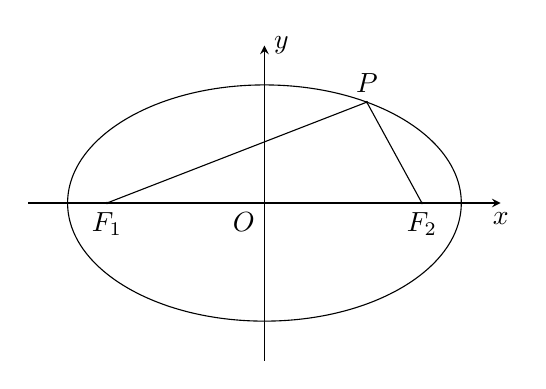
\begin{tikzpicture}
        \pgfmathsetmacro\x{3}
        \pgfmathsetmacro\y{2}
        \pgfmathsetmacro\a{2.5}
        \pgfmathsetmacro\b{1.5}
        \pgfmathsetmacro\c{sqrt(abs(\a^2-\b^2))}
        \pgfmathsetmacro\px{1.3}
        \pgfmathsetmacro\py{sqrt(\b^2*(1-(\px^2)/\a^2))}
        \coordinate (O) at (0,0);
        \coordinate (F1) at (-\c,0);
        \coordinate (F2) at (\c,0);
        \coordinate (P) at (\px,\py);
        \draw[-stealth] (-\x,0) -- (\x,0) node [below] {$x$};
        \draw[-stealth] (0,-\y) -- (0,\y) node [right] {$y$};
        \fill (O) node [below left] {$O$} circle (0.5pt);
        \fill (F1) node [below] {$F_1$} circle (0.5pt);
        \fill (F2) node [below] {$F_2$} circle (0.5pt);
        \fill (P) node [above] {$P$} circle (0.5pt);
        \draw (F1) -- (P) -- (F2);
        \draw (O) circle [x radius=\a,y radius=\b];
    \end{tikzpicture}
\end{document}